\documentclass[dcc]{fcfmcourse}
\usepackage{teoria}
\usepackage[utf8x]{inputenc}
\usepackage{listings}

\renewcommand{\lstlistingname}{Archivo}

\title{Tarea 2: Expansión}
\course[CC3001]{Algoritmos y Estructuras de Datos}
\professor{Nelson Baloian}
\professor{Patricio Poblete}
\assistant{Gabriel Azócar}
\assistant{Manuel Cáceres}
\assistant{Michel Llorens}
\assistant{Sergio Peñafiel}
% Si pasas el comando usedate a la clase, la fecha aparecerá bajo la lista de auxiliares.
% Puedes usar el formato de fecha por defecto de latex (y traducirla usando babel)
% o puedes escribir lo que quieras con el comando \date.
% \date{1 de Septiembre, 2015}

\setlength{\parindent}{0pt}

\begin{document}
\maketitle
\vspace{-2ex}
\begin{center}
Fecha de Entrega: 21 de Abril 23:59hrs
\end{center}

\begin{figure}[h!]
    \centering
    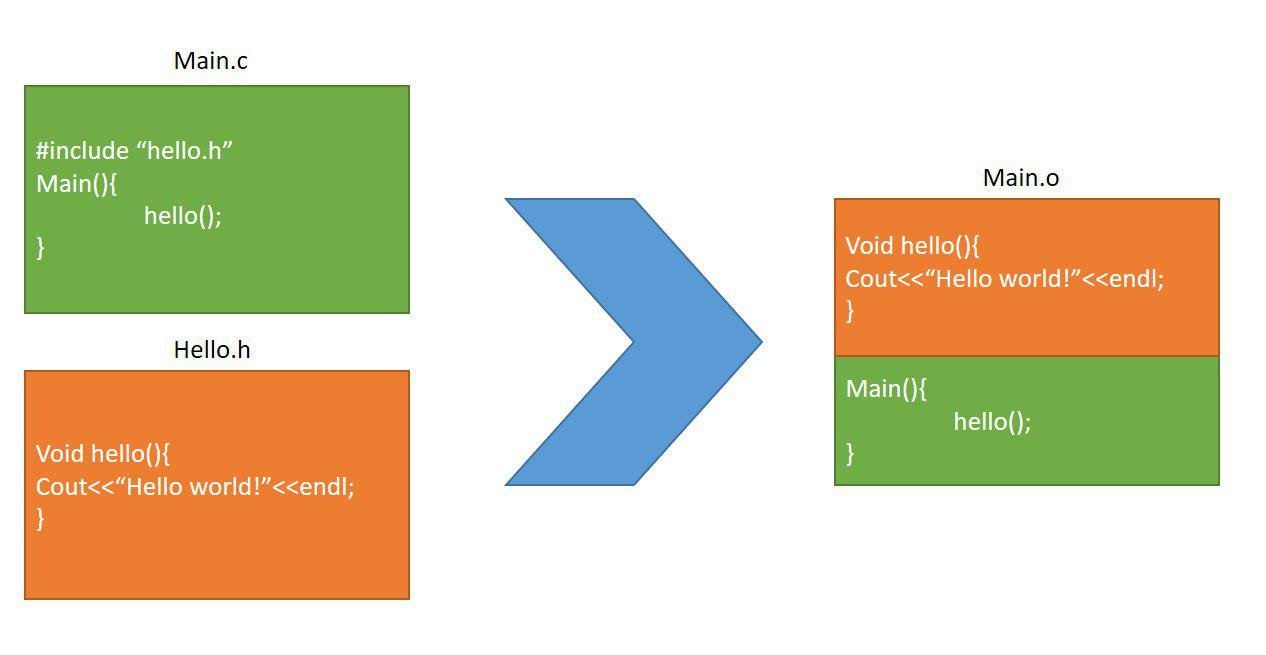
\includegraphics[scale=0.8]{imagenes/diagrama.jpg}
\end{figure}

\section{Introducción}
En la computación, muchas veces al escribir un programa (independiente del lenguaje) uno hace referencia a otros códigos o funciones que suelen estar directamente en otros archivos. Sin embargo, copiar y pegar todo este código al escribir un programa no es conveniente y lo vuelve poco legible.\\

Por tanto, generalmente los lenguajes compilados como lo son Java, C++ y C permiten utilizar referencias a otros archivos, las cuales al momento de compilar se \textbf{expanden} completando con el código correcto. \\

En C, la palabra clave de la referencia es \texttt{\#include <file>}, la cual va sola en una línea y le permite al compilador rellenar ese espacio con el archivo \texttt{file}.

\section{Explicación}

\subsection{Expandir}
Para esta tarea, la idea es crear un programa que funcione tal y como un compilador, es decir, vaya leyendo un archivo y por fácilidad, imprimiendolo en pantalla (utilizando la salida estándar) con todos los reemplazos correspondientes. En nuestro caso las referencias serán denotadas con la forma \textbf{\texttt{<<<nombre\_archivo>>>}}. Un ejemplo de esto es.

\begin{lstlisting}[frame=single, caption={archivo1}]
El archivo 2 dice:\n
<<<archivo2>>>, y el archivo 3\n
dice: <<<archivo3>>>\n
aqui termina el archivo 1.\n
\end{lstlisting}

\begin{lstlisting}[frame=single, caption={archivo2}]
[contenido del archivo 2]\n
\end{lstlisting}

\begin{lstlisting}[frame=single, caption={archivo3}]
El archivo 3 contiene al\n
archivo 4 aqui: <<<archivo4>>>\n
\end{lstlisting}

\begin{lstlisting}[frame=single, caption={archivo4}]
[contenido del archivo 4]\n
\end{lstlisting}


\textbf{Nota:} el char \textbf{\textbackslash n} es un salto de línea (o newline) y no se ve en un archivo y tampoco son dos caracteres distintos. \\

Ahora, el resultado de pasar el archivo1 por nuestro programa de expansión debería mostrar en la salida lo siguiente:

\begin{lstlisting}[frame=single]
El archivo 2 dice:\n 
[contenido del archivo 2]\n 
, y el archivo 3\n
dice: El archivo 3 contiene al\n
archivo 4 aqui:[contenido del archivo 4]\n
\n
\n
aqui termina el archivo 1.\n
\end{lstlisting}

Por términos de eficiencia el programa debería ser capaz de trabajar con un listado de archivos y así no tener que operar de a uno. Por tanto si se le entregan como argumento archivo2 y archivo4 (en ese orden), debería imprimir:

\begin{lstlisting}[frame=single]
[contenido del archivo 2]\n 
[contenido del archivo 4]\n 
\end{lstlisting}

\newpage
\section{Implementación}
En esta tarea usted deberá entregar un archivo \texttt{Expand.java} que recibirá como argumentos de ejecución un listado de nombres de archivos, a los cuales realizará de forma \textbf{recursiva} el proceso de expansión. \\

Se debe tener particular cuidado con las referencias circulares entre los mismos archivos, como lo son $archivo1\Rightarrow archivo2 \Rightarrow archivo3 \Rightarrow archivo1$, ya que estas producirán indudablemente un ciclo infinito de llamadas recursivas y el programa se caerá. Por tanto usted debe detectar estas situaciones y detenerse (evitando así el StackOverFlowException). En caso contrario su programa debería terminar normalmente. \\

La forma en que se ejecutará su programa será desde línea de comando y para ejemplificar, a continuación una ejecución con 3 archivos (podrían ser N):

\begin{lstlisting}[frame=single]
> java Expand archivo1 archivo2 archivo3
\end{lstlisting}

Por facilidad, los archivos se deben encontrar en la misma carpeta que el código. \\


\newpage
\section{Reglas}

\begin{itemize}
    \item Esta tarea debe ser resuelta en Java.
    \item Es obligatorio la entrega de un informe en formato pdf junto con su tarea (Ver siguiente sección).
    \item Esta tarea es de carácter individual, cualquier caso de copia se evaluará con la nota mínima.
    \item No olvide subir a U-cursos \textbf{todos} los archivos necesarios para que su tarea funcione correctamente.
    \item Debe subir los archivos de código fuente (*.java). Los archivos compilados (*.class) no serán evaluados.
    \item Cualquier duda respecto a la tarea puede ser consultada usando el foro del curso.
    \item No se aceptan atrasos.
\end{itemize}

\section{Informe}

El informe debe describir el trabajo realizado, el código fuente desarrollado, los resultados obtenidos y las conclusiones o interpretaciones de estos. Principalmente sea conciso, describiendo cada uno de los puntos que a continuación se indican.

\begin{itemize}
    \item \textbf{Portada:} Indicando número de la tarea, fecha, autor, email, código del curso.
    \item \textbf{Introducción:} Descripción breve del problema y su solución.
    \item \textbf{Análisis del problema:} Exponga en detalle el problema, los supuestos que pretende ocupar, casos de borde y brevemente la metodología usada para resolverlo.
    \item \textbf{Solución del problema:}
    \begin{itemize}
        \item Algoritmos de solución, incluyendo toda la información y figuras que considere necesarias.
        \item Partes relevantes del código fuente
        \item Ejemplos de entradas y salidas escogidos por usted.
    \end{itemize}
    \item \textbf{Modo de uso:} explicando brevemente cualquier dato extra necesario para la compilación y ejecución de su programa.
    \item \textbf{Resultados y análisis:} Todo el análisis de los resultados, los gráficos, imágenes y la discusión requerida.
\end{itemize}

\end{document}